
\chapter{Introduction}

A model specified using the \ac{vdm} can be validated against its
contract-based elements (e.g.\ pre- and postconditions and invariants)
in order to ensure that the system behaves as intended. This can, for
example, be done through model animation using Overture's \ac{vdm}
interpreter.

When sufficient insight into the system under development has been
obtained during the formal analysis, development proceeds to the
implementation phase, where the system is realised. One way to realise
a \ac{vdm} model (which forms the focus of this technical report) is
by implementing it in a programming language using code
generation. However, since no guarantees are currently made about the
correctness of the generated code, other measures must be taken to
increase the confidence in the correctness of the derived model
implementation.

To support this approach, Overture enables fully automated translation
of \vsl's contract-based elements (pre- and postconditions, and
invariants) and type constraints into \ac{jml} annotations. This
translation is achieved using Overture's \emph{\ac{jml} translator},
which translates \ac{vdmsl} models into \ac{jml}-annotated Java
programs. In this way \ac{jml} tools can be used to validate the
generated Java code against the \emph{intended} system behaviour,
described using \ac{jml}. This work-flow is illustrated in
\cref{fig:vdm2jml-overview}.

\begin{figure}[!ht]
  \centering
  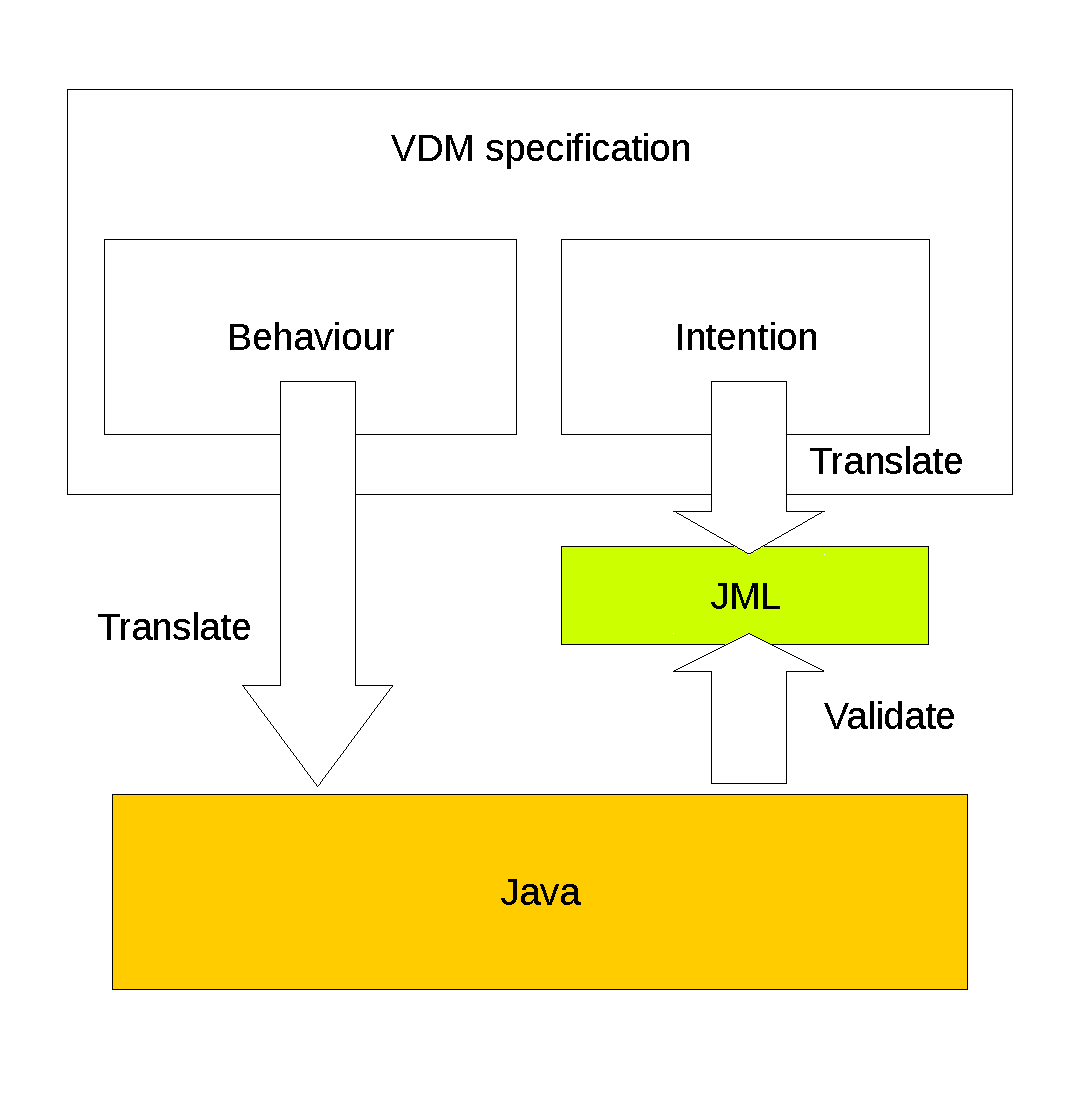
\includegraphics[width=0.6\linewidth]{figs/vdm2jml}
  \caption {Overview of the \ac{vdm}-to-JML translation.}
  \label{fig:vdm2jml-overview}
\end{figure}

\section{The tool implementation}

The translation is defined as a set of rules that are implemented as
an extension of Overture's \ac{vdm}-to-Java code
generator~\cite{Jorgensen&14a} to make the approach fully
automated. The \ac{jml} translator is available in Overture 2.3.8
onwards and can be downloaded via the Overture tool's
website~\cite{Overture}. For instructions on how to use the \ac{jml}
translator we refer the reader to Overture's user
guide~\cite{Larsen&10d}, specifically the chapter on the
\ac{vdm}-to-Java code generator.

The generated Java programs can be checked for correctness using
\ac{jml} tools that support Java 7 or later. In particular, the
generated Java programs, including this translation, have been tested
using the OpenJML~\cite{Cok&11} runtime assertion checker, which at
the current time of writing, supports Java 8. In particular, OpenJML,
is the only \ac{jml} tool that we are aware of that currently supports
all the \ac{jml} constructs generated by the \ac{jml} translator. The
most recent version of OpenJML is available via the OpenJML
website~\cite{OpenJMLWebsite}.

% PJ: To avoid unintentional page break
\newpage

\section{About this technical report}

The purpose of this report is to assist \ac{vdm} users with getting
started using the \ac{jml} translator. Moreover, this report is
complementary to~\cite{Jorgensen&16a} -- a journal paper that
describes the \ac{jml} translation. In that paper, as well as in this
report, the translation is exemplified using a \ac{vdmsl} model of an
\ac{atm}. Due to space limitations only a limited number of examples
are provided in~\cite{Jorgensen&16a}. To improve this, this report
presents a more complete definition of the translation, including more
examples that demonstrate how the translation works.

This report is structured as follows: \Cref{chp:trans} presents the
translation and demonstrates how the \ac{jml} translator supports the
implementation of \vsl models in Java. \Cref{app:atm-model} contains
the complete version of the \ac{atm} model, and the corresponding
Java/JML implementation is available in \cref{app:atm-code}. Finally,
all the regression tests that are used to validate the translation
rules are presented in \cref{app:regression-tests}.

%%% Local Variables:
%%% mode: latex
%%% TeX-master: "../vdm2jml-tr"
%%% End:
